
\subsection{Advanced Load Balancing}

\label{advancedlb}

\subsubsection{Control CPU Load Statistics}

Charm++ programmers can control CPU load data in the load balancing database
before a load balancing phase is started (which is the time when load balancing
database is collected and used by load balancing strategies).

In an array element, the following function can be invoked to overwrite the 
CPU load that is measured by load balancing framework.

\begin{alltt}
   double newTiming;
   setObjTime(newTiming);
\end{alltt}

{\em setObjTime()} is defined as a method of class {\em CkMigratable}, which is
the superclass of all array elements.

The users can also retrieve the current timing that the load balancing runtime
has measured for the current array element. 
 
\begin{alltt} 
   double measuredTiming; 
   measuredTiming = getObjTime(); 
\end{alltt}

This is useful when the users want to derive a new CPU load based on the 
existing one.

\subsubsection{Model-based Load Balancing}

Charm++ programmers can also choose to feed load balancer with their own CPU
timing of each Chare based on certain computational model of the applications.

To do so, first turn off automatic CPU load measurement completely
by setting:

\begin{alltt}
   usesAutoMeasure = CmiFalse;
\end{alltt}

in array element's constructor.

Then the users need to implement the following function to the chare array
classes:

\begin{alltt}
   virtual void CkMigratable::UserSetLBLoad();      // defined in base class
\end{alltt}

This function served as a callback that is called on each chare object when
{\em AtSync()} is called and ready to do load balancing. The implementation of
{\em UserSetLBLoad()} is simply to set the current chare object's CPU load to
load balancer framework. {\em setObjTime()} described above can be used for
this.

\subsubsection{Writing a communication-aware load balancing strategy}

Charm++ programmers can choose an existing load balancing strategy from
Charm++'s built-in strategies(see ~\ref{lbStrategy}) for the best performance
based on the characteristics of their applications. However, they can also
choose to write their own load balancing strategies.

The Charm++ load balancing framework provides a simple scheme to incorporate
new load balancing strategies. The programmer needs to write their strategy for
load balancing based on a instrumented ProcArray and ObjGraph provided by the
load balancing framework. This strategy is to be incorporated within this
function:

\begin{alltt}
void FooLB::work(LDStats *stats) \{
  /** ========================== INITIALIZATION ============================= */
  ProcArray *parr = new ProcArray(stats);
  ObjGraph *ogr = new ObjGraph(stats);

  /** ============================= STRATEGY ================================ */
  /// The strategy goes here
  /// The strategy goes here
  /// The strategy goes here
  /// The strategy goes here
  /// The strategy goes here

  /** ============================== CLEANUP ================================ */
  ogr->convertDecisions(stats);
\}
\end{alltt}

Figure~\ref{fig:ckgraph} explains the two data structures available to the
strategy: ProcArray and ObjGraph. Using these, the strategy should assign new
processors for objects it wants to be migrated through the setNewPe() method.

\begin{figure}[h]
\centering
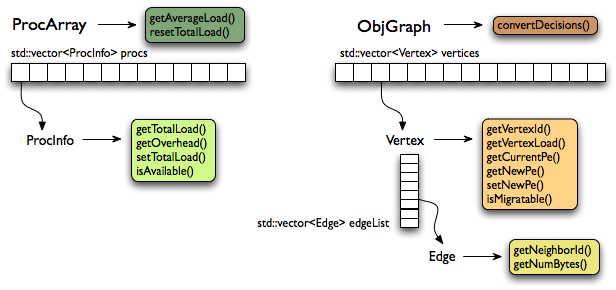
\includegraphics[width=6.0in]{fig/ckgraph}
\caption{ProcArray and ObjGraph data structures to be used when writing a load
balancing strategy}
\label{fig:ckgraph}
\end{figure}

Incorporating this strategy into the Charm++ build framework is explained in
the next section.

\subsubsection{Adding a load balancer to Charm++}

Let us assume that we are writing a new centralized load balancer called FooLB.
The next few steps explain the addition of the load balancer to the Charm++
build system:

\begin{enumerate}
\item Create files named {\em FooLB.ci, FooLB.h and FooLB.C}. One can choose to
copy and rename the files GraphPartLB.* and rename the class name in those
files.

\item Implement the strategy in the {\em FooLB} class method --- {\bf
FooLB::work(LDStats* stats)} as described in the previous section.
%This method takes the load balancing database ({\em stats}) as an input, and
%output the new mapping of objects to processors in {\em stats->to\_proc}
%array.

\item Build charm for your platform (This will create the required links in the
tmp directory).

\item To compile the strategy files, first add {\em FooLB} in the ALL\_LDBS
list in charm/tmp/Makefile\_lb.sh. Also comment out the line containing
UNCOMMON\_LDBS in Makefile\_lb.sh.  If FooLB will require some libraries at
link time, you also need to create the dependency file called
libmoduleFooLB.dep. Run the script in charm/tmp, which creates the new Makefile
named ``Make.lb''.

\item Run ``make depends'' to update dependence rule of Charm++ files.  And run
``make charm++'' to compile Charm++ which includes the new load balancing
strategy files.
\end{enumerate}


\subsubsection{Understand Load Balancing Database Data Structure}

\label{lbdatabase}

To write a load balancing strategy, one may want to know 
what information is measured during the runtime and how it is represented in
the load balancing database data structure?

There are mainly 3 categories of information: a) processor information including processor speed, background load; b) object information including per object
cpu/wallclock compute time and c) communication information .

The database data structure named {\kw LDStats} is defined in {\em CentralLB.h}:

\begin{verbatim}

  struct ProcStats {  // per processor
    LBRealType total_walltime;
    LBRealType total_cputime;
    LBRealType idletime;
    LBRealType bg_walltime;
    LBRealType bg_cputime;
    int pe_speed;
    double utilization;
    CmiBool available;
    int   n_objs;
  }

  struct LDStats { // load balancing database
    ProcStats  *procs;
    int count;

    int   n_objs;
    int   n_migrateobjs;
    LDObjData* objData;

    int   n_comm;
    LDCommData* commData;

    int  *from_proc, *to_proc;
  }

\end{verbatim}

\begin{enumerate}
\item {\em LBRealType} is the data type for load balancer measured time. It is "double" by default. User can specify the type to float if wanted at Charm++ compile time. For example, ./build charm++ net-linux-x86\_64 {-}{-}with-lbtime-type=float;
\item {\em procs} array defines processor attributes and usage data for each
processor;
\item {\em objData} array records per object information, {\em LDObjData} is defined in {\em lbdb.h};
\item {\em commData} array records per communication information. {\em LDCommData} is defined in {\em lbdb.h}.
\end{enumerate}

